% -*- latex -*-
%-----------------------------------------------------------------------
%;  Copyright (C) 2011
%;  Associated Universities, Inc. Washington DC, USA.
%;
%;  This program is free software; you can redistribute it and/or
%;  modify it under the terms of the GNU General Public License as
%;  published by the Free Software Foundation; either version 2 of
%;  the License, or (at your option) any later version.
%;
%;  This program is distributed in the hope that it will be useful,
%;  but WITHOUT ANY WARRANTY; without even the implied warranty of
%;  MERCHANTABILITY or FITNESS FOR A PARTICULAR PURPOSE.  See the
%;  GNU General Public License for more details.
%;
%;  You should have received a copy of the GNU General Public
%;  License along with this program; if not, write to the Free
%;  Software Foundation, Inc., 675 Massachusetts Ave, Cambridge,
%;  MA 02139, USA.
%;
%;  Correspondence concerning AIPS should be addressed as follows:
%;          Internet email: aipsmail@nrao.edu.
%;          Postal address: AIPS Project Office
%;                          National Radio Astronomy Observatory
%;                          520 Edgemont Road
%;                          Charlottesville, VA 22903-2475 USA
%-----------------------------------------------------------------------
%Body of final AIPSletter for 31 December 2011

\documentclass[twoside]{article}
\usepackage{graphics}

\newcommand{\AIPRELEASE}{December 31, 2011}
\newcommand{\AIPVOLUME}{Volume XXXI}
\newcommand{\AIPNUMBER}{Number 2}
\newcommand{\RELEASENAME}{{\tt 31DEC11}}
\newcommand{\OLDNAME}{{\tt 31DEC10}}
\newcommand{\NEWNAME}{{\tt 31DEC12}}

%macros and title page format for the \AIPS\ letter.
\input LET98.MAC

\newcommand{\MYSpace}{-11pt}

\normalstyle

\section{General developments in \AIPS}

\subsection{Current and future releases}

We have formal \AIPS\ releases on an annual basis.  We recommend a
full binary installation method for both the frozen and development
versions for MacIntosh OS/X (PPC and Intel chips), Solaris, and Linux
(32- and 64-bit) systems, but all architectures can do a full
installation from the source files.  If you develop \AIPS\ code
locally, you will need to do a source-level installation.  The current
release is called \RELEASENAME\ and is now ``frozen.''  If you took a
development copy of this version at some earlier date, you should use
the ``Midnight Job'' (MNJ) to bring it up to date.  You need to run a
MNJ only once in 2012 to convert your copy of \RELEASENAME\ into the
frozen version.  However, when patches to \RELEASENAME\ are announced,
you may apply them with the MNJ\@.  This \Aipsletter\ is intended to
advise you of corrections and improvements in this release.

We have begun a new version, called \NEWNAME, which is now under
development by the \AIPS\ Group.  You may fetch and install a complete
copy of this version at any time.  Having fetched \NEWNAME, you may
update your installation whenever you want by running the MNJ\@.  This
uses cvs, rsync, and/or transaction files to copy and compile the code
selectively based on the code changes and compilations we have done.
We expect users to take their source-only or binary version of
\NEWNAME\ \AIPS\ over the Internet (via \emph{anonymous} ftp).  Both
versions require you to copy the installation procedure {\tt
install.pl} via {\tt ftp}; the source-only version also requires you
to ftp the 112-Mbyte {\tt \NEWNAME.tar.gz} compressed tar file.  Linux
sites will almost certainly have {\tt cvs} installed; other sites may
have installed it along with other GNU tools.  Secondary MNJs will
still be possible using {\tt ssh} or {\tt rcp} or NFS as with previous
releases.  We have found that {\tt cvs} works very well, although it
has one quirk.  If a site modifies a file locally but in an
\AIPS-standard directory, {\tt cvs} will detect the modification and
attempt to reconcile the local version with the NRAO-supplied version.
This usually produces a file that will not compile or run as intended.

\AIPS\ is now copyright \copyright\ 1995 through 2011 by Associated
Universities, Inc., NRAO's parent corporation, but may be made freely
available under the terms of the Free Software Foundation's General
Public License (GPL)\@.  This means that User Agreements are no longer
required, that \AIPS\ may be obtained via anonymous ftp without
contacting NRAO, and that the software may be redistributed (and/or
modified), under certain conditions.  The full text of the GPL can be
found in the \texttt{15JUL95} \Aipsletter\ and is included with every
distribution in file {\tt \$AIPS\_ROOT/{\it release-name}/COPYING}\@.
\vfill\eject

\subsection{\Aipsletter\ publication}

We have decided to discontinue paper copies of the \Aipsletter\ other
than for libraries and NRAO staff.  The \Aipsletter\ will be available
in PostScript and pdf forms as always from the web site listed above
and included in all \AIPS\ installations.  It will be announced in the
NRAO e-News mailing and on the bananas and mnj list servers.

\subsection{Installing a new version}

If compiling locally, new releases must be installed from the tar ball
for that release.  If using the binary installation, a full new
installation must also be done with {\tt rsync}.  The {\tt cvs} system
requires this.  When installing a new \AIPS\ release in a system that
already has a previous release, we recommend that {\tt install.pl} be
used and that the previous release be left in place, at least until
the new installation has been verified.  If you do this, then you will
not have to re-edit the disk, printer, and tape lists and can simply
skip all those pages in the {\tt install.pl} menus.  The old {\tt
  \$HOME/.AIPSRC} file may be left in place, but it will need to be
edited.  The lines giving the {\tt DOWNLOADED} and {\tt UNPACKED}
parameters should be cleared and the {\tt CCOMOPT} line should be
changed to point to the current release rather than the previous one.
If you have made a special version of {\tt do\_daily.{\it host}}, you
should preserve it under a new name and restore it after the install.
If you have an odd set of \AIPS\ versions, the {\tt
  \$AIPS\_ROOT/AIPSPATH.*SH} files may need to be edited after the
install to set the desired versions.


\section{\AIPS\ Distribution}

From the NRAO system logs, we count apparent MNJ accesses, downloads
of the tar balls, and {\tt rsync} accesses by unique IP address.
Since DSL and some university and other connections may be assigned
different IP addresses at different times, this will be a bit of an
over-estimate of actual sites.  However, a single IP address is often
used to provide \AIPS\ to a number of computers, so these numbers are
at the same time an under-estimate of the number of computers running
current versions of \AIPS\@.  In 2011, a total of 270 different IP
addresses downloaded the frozen form of \OLDNAME\ and 1105 IP
addresses downloaded \RELEASENAME\ in tarball or binary form.  Fully
1747 IP addresses accessed the NRAO cvs master.  Each of these has at
least installed some version of \AIPS\ and many appear to have run the
MNJ at least occasionally.  The total number of unique IP addresses in
these three lists was 2228.  424 sites accessed \OLDNAME\ in binary
form, while 1064 sites used the binary form of \RELEASENAME\@.  The
attached figure shows the cumulative number of unique sites, cvs
access sites, and tar-ball/binary download sites known to us as a
function of week in 2011.  The numbers for 2010 are also plotted and
show that there has been about a 10\%\ drop this year beginning in the
middle of the year.  Presumably {\tt CASA} is responsible for this.

%\centerline{\resizebox{4.8in}{!}{\includegraphics{FIG/PLOTIT11b.PS}}}
\centerline{\resizebox{!}{3.0in}{\includegraphics{FIG/PLOTIT11b.PS}}}

\vfill\eject

\section{Preview of coming attractions}

The \NEWNAME\ release already contains a few changes that we decided
were a bit risky or not needed in \RELEASENAME\@.  {\tt LISTR} will
print {\tt SY} tables as {\tt OPTYPE='GAIN'}, showing the apparent
system temperature or the gains that {\tt TYAPL} will apply.  TV code
was changed generally to try to avoid having tasks that are failing
end up hanging waiting on the TV display.  Handling of the {\tt CQ}
table --- used to correct VLBI data for decorrelation occurring in the
correlator --- has been corrected for large FFT sizes with uniform
taper; related error messages were clarified.

\section{Improvements of interest to users in \RELEASENAME}

We expect to continue publishing the \Aipsletter\ every six months
along with the annual releases.  There are a few new tasks released in
the last six months.  New tasks include {\tt REFLG} to compress flag
tables, {\tt FGDIF} to compare two flag tables, {\tt SNIFS} to plot
table values versus IF, {\tt RFARS} to correct polarization cubes for
rotation measure found in {\tt FARS}, and {\tt NANS} to examine data
sets and images for NaNs (not-a-number) and magic-value blanks.  A
{\tt QCREATE} adverb was added to {\tt GO} to request that data files
be created in a fast method that does not guarantee that the disk
space will actually be available when needed.

In the first six months of \RELEASENAME\ the new tasks were {\tt
  REWGT} to scale data weights by subarray and/or IF, {\tt ACLIP} to
do clip operations on auto-correlation data, {\tt RLCAL} to solve for
right minus left phase differences as a function of time when good
source models are available, {\tt SY2TY} to make {\tt TY} tables from
SysPower tables, {\tt SYCOP} to copy good {\tt SY} table IFs to bad
ones, {\tt QUOUT} and {\tt QUFIX} to determine right-left calibrations
from well-calibrated images, {\tt RFLAG} to flag data based on rmses
measured over short time intervals and on deviations from the spectral
average, {\tt IM2CC} to convert model images into Clean components
attached to suitable image facets, and {\tt AFARS} to extract useful
parametric images from the Faraday Rotation synthesis ({\tt FARS})
output image cubes.  The new verb {\tt HUEWEDGE} draws a step wedge in
two dimensions on the TV and even labels it to match a {\tt TVHUEINT}
display.  The OBIT programs {\tt BDFIn} and {\tt BDFList} have been
made accessible to \AIPS\ users through ``verbs'' {\tt BDF2AIPS} and
{\tt BDFLIST}.  These replace earlier stand-alone, question-and-answer
scripts far translating EVLA SDM data sets.  This worked so well that
further ``verbs'' {\tt OBITMAP}, {\tt OBITIMAG}, {\tt OBITSCAL}, and
{\tt OBITPEEL} have been written to make available increasingly
complex portions of the OBIT program {\tt Imager}.  All of these verbs
require the {\tt OBIT} package to be installed on the computer.  A new
pipeline procedure named {\tt DOOSRO} has been written to reduce EVLA
data taken with less difficult observing parameters (``Open shared
risk'').  A service program to list assigned user numbers called {\tt
  USERNO} was re-created.

Normally, bugs which are created in an \AIPS\ {\tt TST} version and
then fixed in that same version before its release get little or no
discussion in the \Aipsletter\@.  Since a rather large number of sites
now install the {\tt TST} version of \AIPS\ during its development,
this is somewhat of an oversight.  We urge you to run the ``Midnight
Job'' at least once after \RELEASENAME\ is frozen to bring it up to
date and to fix all bugs of this sort.  We urge active sites to use
the MNJ and, when something odd occurs, to examine {\tt CHANGE.DOC}
using the cgi tool available from the \AIPS\ web page under
documentation.  Please do not hesitate to e-mail {\tt daip@nrao.edu}
with any questions or suspicions that there are problems.

{\tt 31DEC09} contains a change in the format of antenna files.
Previous releases will not understand the antenna coordinates for
arrays that were traditionally left-handed (VLBI primarily).  The
format change occurs automatically when any {\tt 31DEC09} or later
antenna-file specific code reads the file, after which older releases
will have difficulties.  Note that the only version which we patch for
major errors is \RELEASENAME; even \OLDNAME\ is no longer changed.

\subsection{UV data}

\subsubsection{RFLAG}

RFI is frequently characterized by rapid variability in both time and
frequency.  The relatively new task {\tt RFLAG} looks for this and
flags the data accordingly.  It received a great deal of attention in
the last 6 months and has become the most important flagging task for
EVLA data.  Using a floating buffer in time (usually just 3 or 5
integrations), {\tt RFLAG} measures the rms over time in each channel
individually.  If the rms exceeds a cutoff, the channel is flagged
over that time range.  {\tt RFLAG} also finds the mean and rms of the
real and imaginary parts of the visibility over the channels in each
spectral window at each time.  The task uses ``robust'' methods which
exclude outliers while finding the ``real'' mean and rms.  Any channel
that deviates by more than a cutoff in Jy will also be flagged.  To
assist in setting the time and spectral cutoffs, {\tt RFLAG} can plot
the spectrum of the mean time and spectral rms in each channel and
their variance.  It uses these to return suggested cutoffs as a
function of spectral window (IF)\@.  It can also plot the histograms
of values of the time rms and the spectral deviations.  The task can
now do plots finding cutoff levels followed optionally by applying
those levels, or it can apply input cutoffs to the data and then
optionally make plots showing the results of applying the new flag
table.

{\tt RFLAG} has numerous options to do additional flagging beyond the
direct application of the cutoffs.  It can flag up to $n$ channels
between groups of flagged channels.  It can flag a channel over all
baselines if too large a fraction are flagged by the cutoffs or flag a
full spectral window if too many channels are flagged.  It also
applies a clip operation prior to examining the data for the rmses.
{\tt RFLAG} can write a text file with channel weights based on the
rmses over time and/or over channel.

{\tt RFLAG} can produce enormous numbers of flags.  The new task {\tt
  REFLG} was written to attempt to compress the flag table by merging
channels and time intervals primarily, although it attempts other
compressions as well.  {\tt REFLG} offers some of the flag extension
options of {\tt RFLAG} plus one, which is not available to {\tt
  RFLAG}, to flag all times for a channel if too large a fraction of
the times are flagged.  The new task {\tt FGDIF} was written to
compare the consequences of two different flag tables and was
important in debugging {\tt REFLG}\@.

\subsubsection{EVLA-driven changes}
\begin{description}
\myitem{PCAL} was changed to make an intermediate file of the current
           spectral window prior to selecting the data for each channel.
           This can speed up the task by factor of 8 or more.  It was
           revised to handle indeterminate solutions in one or more
           spectral channels without quitting and to deal with a fully
           flagged IF\@.  It was changed to force the needed status
           when writing the solution tables and to set {\tt SOLINT} to
           1/3 of a scan when only one scan is requested.
\myitem{TYAPL} was corrected to do the best possible job of
           interpolation in the presence of extensive flagging in the
           {\tt SY} or {\tt TY} table.  It can now apply to the $uv$
           data up to 200000 flags applying to a single time.
\myitem{SETJY} was using the reference channel for the frequency at
           which the flux of each IF was computed.  This is not
           representative if the reference channel is channel 1.
           An option to chose the channel for the flux was added, with
           the center of the IF as the default.
\myitem{SPLAT} was changed to apply any flagging to {\tt SY}, {\tt
           TY}, and {\tt SN} tables that are copied.
\myitem{UVCOP} was changed to apply any flagging to {\tt SY}, {\tt
           TY}, and {\tt SN} tables that are copied.  It was changed
           to use the index table to speed its operations.  The
           flagging for low weights option was made correct and
           meaningful.  Previously it dropped full records if
           everything was of low weight, but did not flag low weights
           when some of the record had higher weight.  A bug was
           corrected that caused {\tt UVCOP} with {\tt SOURCES}
           specified to fail to flag any $uv$ or table data.
\myitem{TVFLG} and {\tt SPFLG} were changed to use the calibration and
           index tables while finding the times for the work file,
           greatly speeding that operation in some cases.  They use greater
           precision in displaying times when appropriate.  They were
           corrected to display and flag Stokes types compounded from
           the input (such as I, V from RR and LL) as requested.  In
           such cases, all input Stokes are flagged.  {\tt TVFLG} was
           given a {\tt FLAG BASELINE-DT} operation.
\myitem{Warnings} about failure to reference one antenna to another
           were corrected generally.  Now, if the message appears,
           it is a real problem rather than a confusion over IFs,
           polarizations, subarrays, etc.
\myitem{RLDLY} was changed to copy only the necessary baselines and to
           use the index table when finding integration times, making
           it rather faster.  An abort only on Macs was corrected.
           {\tt PRTLEV} was added to allow diagnostics when the
           solutions fail.
\myitem{CLCAL} failed to reference phases properly when smoothing to
           replace failed solutions.  Corrected it to use the
           reference data of the good solutions being smoothed.
\myitem{CALIB} was changed to forbid {\tt DOCAL} true for
           single-source files since that would force a multiplication
           of 2 {\tt SN} tables.
\myitem{REWGT} was given the option of reading a text file of channel
           weights to apply to the data.  {\tt RFLAG} is able to make
           such a file from the time rmses.
\myitem{FLOPM} copied tables only over the time range being
           ``flopped'' although all $uv$ data were copied.
\end{description}

\subsubsection{Other changes}
\begin{description}
\myitem{DOBAND} was incorrect for auto-correlation data.  Only the
           real part of the bandpass was applied.  The normal
           cross-correlation correction function is what is actually
           needed.
\myitem{MC table} times are actually start times not midpoint times
           despite indications to the contrary.  This led to errors in
           the {\tt CL} table version 1 values for clock and
           atmosphere in the correlator model for VLBI data.
\myitem{FRING} was changed to faster methods of disk I/O when
           determining the integration time at the beginning.  The
           multi-band delay was set erroneously in the EVLA mode.
           Error messages about excessive FFT size were clarified.
           The code was corrected to work for up to 90 antennas, like
           the rest of \AIPS\@.
\myitem{USUBA} had internal limits on {\tt NX} table entries, number
           of sources, and number of antennas.  Changed these to
           much larger values.
\myitem{VPFLG} was changed to add meanings to the adverb {\tt DOIFS}
           to allow extending the flagging to an IF or even all IFs.
\end{description}

\subsection{Imaging}

{\tt IMAGR} could get confused, when {\tt ONEBEAM} was true, about
what Clean beam size to use when scaling a particular plane of an
output cube.  The beam used was correctly recorded in the {\tt CG}
table, but the planes were scaled oddly.  The code was corrected to
allow {\tt ALLOKAY} to function properly when doing baseline-length
dependent time averaging on the fly.  The code was rearranged to loop
over {\tt SUBARRAY} to allow all sub-arrays to be used even with
calibration and flagging.  The TV timeout periods may now be
controlled with adverbs {\tt IM2PARM(8) and (9)}\@.

\subsection{Analysis}

\begin{description}
\myitem{RFARS} is a new task to apply the rotation measures found by
           {\tt FARS} and {\tt AFARS} to the original input cubes.
           Weak polarization signals may then be averaged to improve
           the signal-to-noise.
\myitem{SQASH} was re-written.  Modern disk systems do not work well
           with the old I/O methods, which once were fine.  Added was
           the ability to find data weights (robustly) from the image
           planes or by reading a text file in order to make weighted
           mean and weighted rms images.  {\tt SQASH} was changed to
           allow squashing even axis 2, producing interesting
           one-dimensional and, \eg\ position-velocity images summed
           over the other spatial coordinate.
\myitem{IMEAN} was changed to compute an initial guess for fitting the
           true rms from a robust method rather than using the {\tt
             PIXSTD} and {\tt PIXAVG} adverbs.  These are now purely
           output adverbs from the task.
\myitem{CONVL} now examines the header and {\tt CG} table and
           convolves a cube if any channel will convolve to the
           desired resolution.  It fills with magic blanks any channel
           that cannot be convolved to the desired resolution.
\myitem{XMOM} was given a new {\tt OPTYPE = 'MAX'} to make images of
           the maximum pixel value and its location rather than the
           moment sums.  This reveals additional interesting aspects
           of spectral-line cubes.
\vfill\eject
\myitem{UVFIT} was given the ability to read an {\tt INLIST} text file
           for initial guesses of up to 20 components.  The file may
           contain guesses for multiple spectral channels but only
           those matching {\tt BCHAN} are used.  The number of
           visibilities allowed was raised by a lot and the default
           {\tt GMAX} was corrected since a value of 0.0 caused the
           task to fail to iterate.  A compact text-file output was
           added and the task's messages were changed to be more
           readable.
\myitem{STFUN} now writes out an ``rms'' image along with the
           structure function image.  The statistics are not simple
           Gaussian since the function is already squared, but the rms
           image is still indicative.
\end{description}

\subsection{Display}

\begin{description}
\myitem{SNIFS} is a new task to plot tables as a function of IF\@.  It
           has numerous options controlling time averaging and the
           plotting of multiple things in a panel, but can still
           generate a great many plots.
\myitem{PRTAB} now uses {\tt RPARM} to do up to 7 tests on a row to
           decide whether to display it or not.  The handling of the
           string comparison test was corrected.  The task no longer
           reads all of large files to decide on column formats and
           makes somewhat better decisions about those formats.
\myitem{ISPEC} now offers the option of natural and base-10
           logarithmic vertical scales and options to plot the linear
           derivative of its basic plots.  The latter is especially
           helpful for Zeeman experiments.
\myitem{Stars} files may now be written containing the fit results of
           {\tt SAD}, {\tt IMFIT} and {\tt JMFIT}\@.  New adverb {\tt
             STVERS} is used by the plot tasks to control the plotting
           of the ``stars.''
\myitem{VPLOT,} {\tt CLPLT}, and {\tt CAPLT} were changed to allow up
           to 200000 Clean components in models and were corrected to
           handle more than 64 fields properly.  {\tt VPLOT} was also
           changed to allow a mammoth number of visibilities.
\myitem{POSSM} and {\tt BPLOT} were given options to plot the
           difference between right-hand and left-hand polarization
           bandpasses.
\myitem{TVHELIX} was given the {\tt DOPRINT} option to provide a
           display of its parameters.  This may help to refine one's
           setting of this rather complicated coloring scheme.
\end{description}

\subsection{General and system matters}

\begin{description}
\myitem{UBUNTU} 11.04 systems have shown a variety of odd issues.
           Apparently X-Windows is not the default screen manager, but
           needs to be selected to enable \AIPS\ display windows to
           function.  These windows can get ``lost'' if they start in
           icon form.  {\tt XAS} was changed to start open, with an
           {\tt .XDefaults} option to start in icon form.  The {\tt
             TEK} and {\tt MSG} windows were each given an environment
           variable that can cause them to start open and in {\tt
             -hold} mode.  The latter means the windows do not die
           when the \AIPS\ program in them terminates.  The help files
           for {\tt XAS}, {\tt TERKSRV}, and {\tt MSGSRV} provide
           details.
\myitem{QCREATE} is a new adverb to {\tt GO}\@.  It specifies that
           file creations should be done quickly, rather than by
           filling the full file with zeros.  This runs the risk that
           the disk space will not actually be available when needed,
           but can be a great deal faster.
\myitem{FITTP} and {\tt FITAB} were changed to avoid interpreting any
           floating-point values in $uv$ data sets as magic blanks.
           Previously it was possible for $uv$ and data values equal
           to the ``magic value'' (3140.89282 on byte-swapped
           computers) to occur and be written as NaNs (not-a-number)
           in the output FITS file.  This worked okay when the file
           was read back into \AIPS, but not when it was read by other
           packages.
\myitem{NANS} is a new task designed to look for NaNs and magic blanks
           in \AIPS\ files.  It was written to explore data sets and
           tables with potential problems.
\myitem{CookBook} was updated including a new Appendix (E) specifically
           addressed to EVLA users.
\myitem{Return} adverbs from tasks were changed so that tasks might
           do the return at an appropriate point and then continue to
           operate.  Previously, {\tt AIPS} waited for the task to
           finish and then looked for the adverbs.
\myitem{Table} sorting code was changed to use dynamic memory in an
           attempt to do as much as possible in memory.  This should
           be faster and simplifies the use of {\tt TABSRT} in tasks.
           Larger disk I/O calls are now allowed by the lowest level
           routines to support this.  {\tt TABSRT} now allows the use
           of array columns as the sort keys, where the calling
           routine specifies which index in the array(s) is to be
           used.
\end{description}


\section{Patch Distribution for \OLDNAME}

Because of the extensive use of binary installations, we now patch the
master copy of the most recently frozen version.  Older versions are
not corrected even for egregious errors.  Thus, \OLDNAME\ was patched
during 2011 and \RELEASENAME\ will be patched as needed during 2012.
Your copy of them may be corrected simply by running a Midnight Job.
Information about patches and the code may be found using links from
the main \AIPS\ web page or by  {\it anonymous} \ftp\ to the NRAO
server {\tt ftp.aoc.nrao.edu}.  Documentation about patches to a
release is placed on this site at {\tt pub/software/aips/}{\it
  release-name} and the code is placed in suitable sub-directories
below this.  Patches to older releases are kept here as well, but they
will require local compilation.

The \OLDNAME\ release is no longer available for installation and will
no longer receive patches even for egregious errors.  It had a number
of important patches during 2011.  They are
\begin{enumerate}
  \item\ {\tt UVCOP} used only 12 of the 16 characters of the {\tt
    SOURCE} adverbs {\it 2011-01-18}
  \item\ {\tt DBCON} was vulnerable to errors in table headers causing
    absurd disk file size expansions. {\it 2011-01-18}
  \item\ {\tt FRING} got wrong answers from the exhaustive search
    method for IFs higher than 1. {\it 2011-01-21}
  \item\ OOP-based $uv$ tasks could write to the wrong output file. {\it
    2011-01-21}
  \item\ {\tt CALIB} failed to build the output header correctly for
    non-standard single-source data sets. {\it 2011-01-24}
  \item\ {\tt RLDIF} did not handle one source, continuum corrections
    properly {\it 2011-01-24}
  \item\ {\tt SWAPR} ignored autocorrelation data. {\it 2011-01-24}
  \item\ {\tt SNPLT} did not handle {\tt PC} table phases correctly.
    {\it 2011-03-23}
  \item\ {\tt IMAGR} did not average multi-channel data correctly when
    doing on-the-fly baseline-length time averaging. {\it 2011-04-15}
  \item\ {\tt NX} tables were written incorrectly when there were
    multiple subarrays. {\it 2011-04-25}
  \item\ {\tt IMEAN} did not write the text file output correctly.
    {\it 2011-06-08}
  \item\ {\tt NOIFS} scaled $uvw\/$'s incorrectly. {\it 2011-06-14}
  \item\ {\tt CVEL} did not die when it should on fatal errors {\it
    2011-06-23}
  \item\ {\tt FITLD} and friends did not read table header
    character-valued keywords correctly. {\it 2011-06-24}
  \item\ {\tt UVCOP} did not apply flags when {\tt SOURCES} was
    specified.  {\it 2011-07-01}
  \item\ {\tt IMAGR} did not keep the correct Clean beams for facets
    other than one when making an image cube with {\tt ONEBEAM} true.
    {\it 2011-07-25}
  \item\ {\tt VPLOT} did not plot models correctly for more than 64
    facets. {\it 2011-07-29}
  \item\ {\tt CLCOR} used the wrong sign of the antenna Y position for
    the {\tt EOPS} and {\tt SUND} operations. {\it 2011-08-04}
\end{enumerate}
\vfill\eject

% Order form and mailer page
%\cleardoublepage
\pagestyle{empty}
%\vfill
%\centerline{\resizebox{!}{23.3cm}{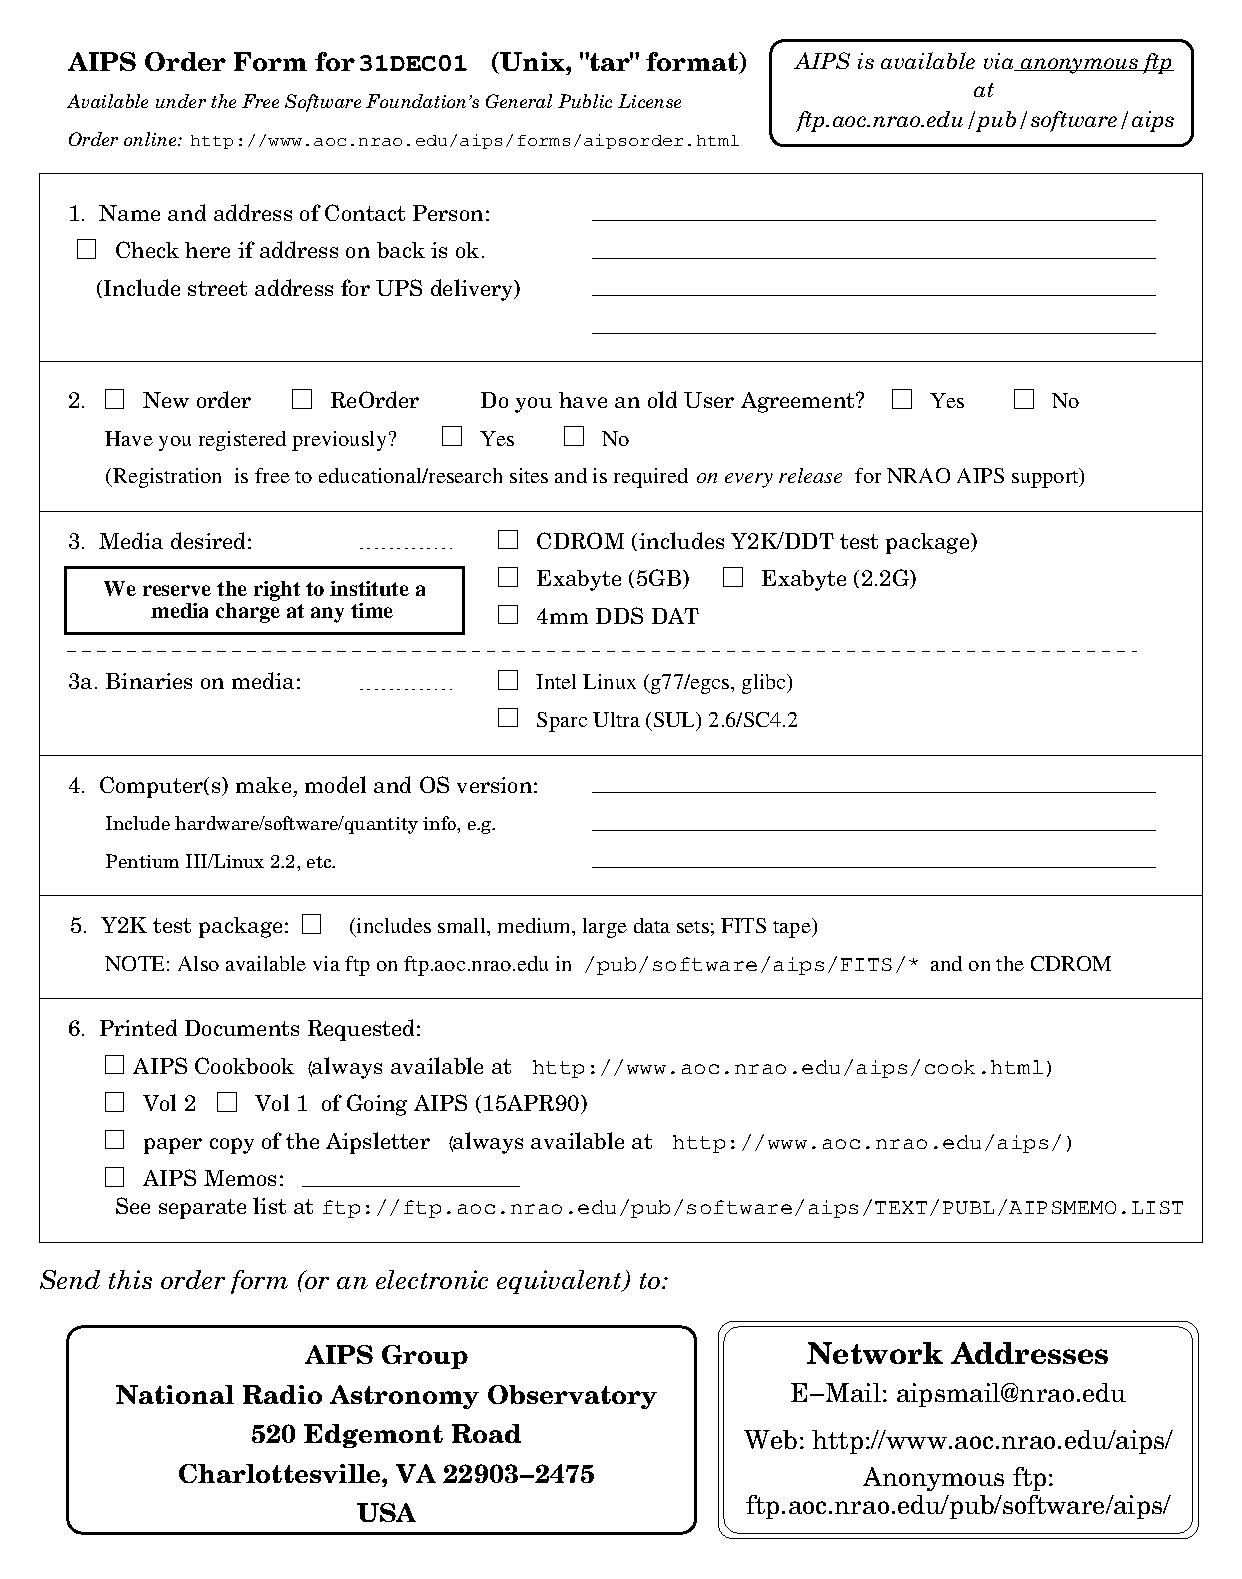
\includegraphics{FIG/AIPSORDER.PS}}}
%\vfill\eject
\vbox to 4.4in{
\vspace{12pt}
%\centerline{\rotatebox{-90}{\resizebox{!}{3.5in}{%
%\includegraphics{FIG/Mandrill.color.plt}}}}
\centerline{\resizebox{!}{3.5in}{\includegraphics{FIG/Mandrill.eps}}}
\vspace{12pt}
\centerline{{\huge \tt \AIPRELEASE}}
\vspace{12pt}
\vfill}
\phantom{...}
\centerline{\resizebox{!}{!}{\includegraphics{FIG/AIPSLETS.PS}}}

\end{document}
